\section{Theory}
\label{sec:theory}
\subsection{The ATLAS experiment}
The ATLAS experiment is one of the four main experiments at the Large Hadron Collider (LHC) at CERN.
The CERN nuclear research center in Geneva reasearches the fundamental structure of matter.
For that purpose,
the LHC accelerates protons in a circular path with a circumference of 27 km to nearly the speed of light.
At the four big experiments (ATLAS, CMS, ALICE, LHCb), 
the accelerated protons collide with each other.

\autoref{fig:Atlas} shows a schematic drawing of the detector in ATLAS. 
\begin{figure}
	\centering
	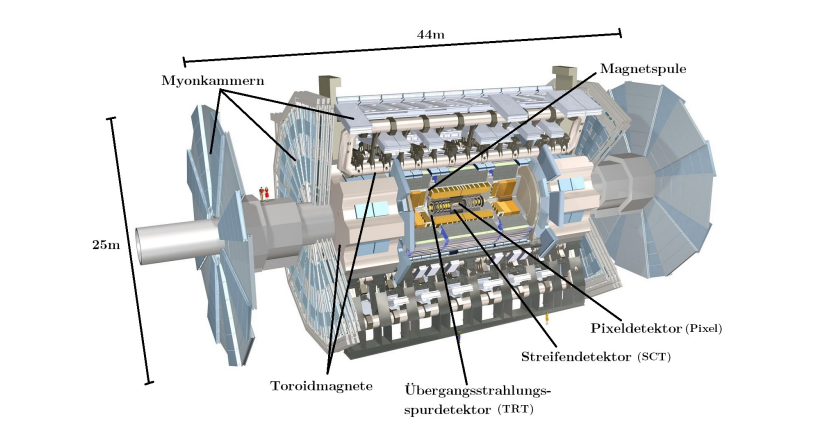
\includegraphics[width=0.8\textwidth]{figure/Atlas.PNG}
	\caption{Schematic drawing of the detector in ATLAS\cite{Vorlage}}
	\label{fig:Atlas}
\end{figure}
The detector is built cylindrically around the collision point of the protons.
So it can detect the particles around an angle of $360^\circ$ around the collision point.
Directly around the collision point is the inner detector.
Its task is to track the primary and secondary vertices that are produced in the collision.
To do that,
the inner detectror needs a high spatial resolution. Therefore, the intermost layer of the inner detector is build with silicon pixel detectors.
Because pixel detectors are very expensive, 
the outer layers of the inner detector are build with silicon strip detectors.
They have a lower spatial resolution but are cheaper to produce.
The inner detector is surrounded by a solenoid magnet that produces a magnetic field.
In this the path of charged particles is bent.
Through the curvature of the path, the momentum of the particles can be determined.

Outside the inner detector are the electromagnetic and hadronic calorimeters.
They measure the energy of the particles by absorbing them.



\subsection{Semiconductor}

\begin{figure}[h]
	\centering
	\begin{subfigure}{0.4\textwidth}
		\centering
		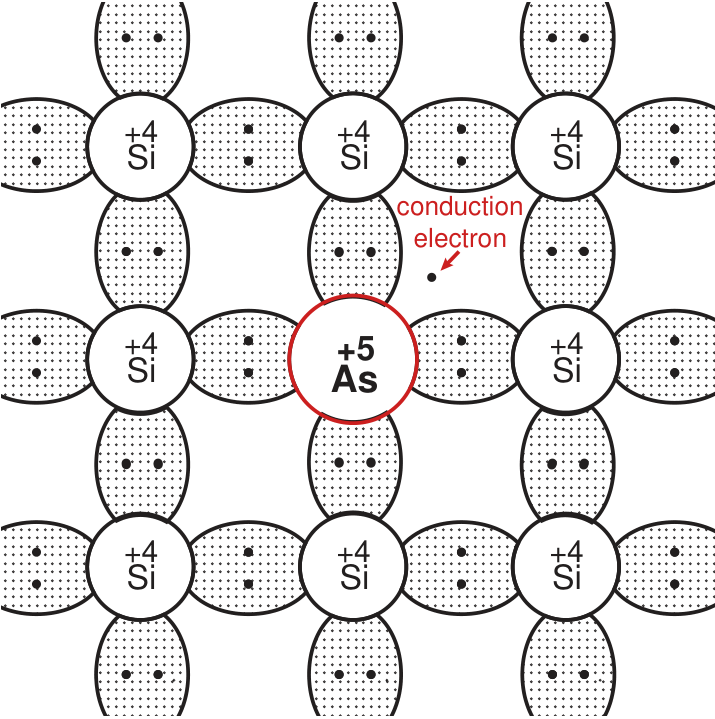
\includegraphics[width=\textwidth,height=5cm]{figure/n_dope}
		\caption{n-type doping}
		\label{n_dot}
	\end{subfigure}
	\begin{subfigure}{0.4\textwidth}
		\centering
		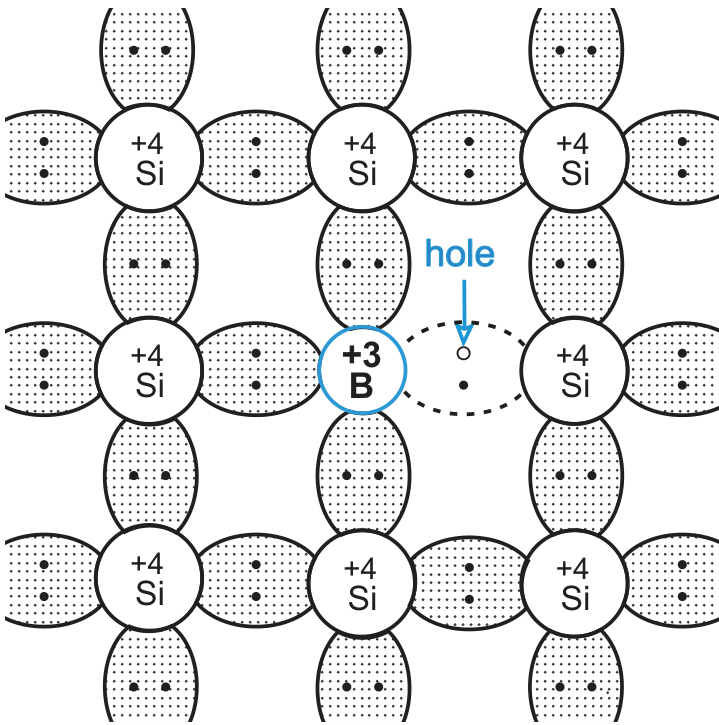
\includegraphics[width=\textwidth,height=5cm]{figure/p_dope}
		\caption{p-type doping}
		\label{p_dot}
	\end{subfigure}
	\caption[Illustration of n-type and p-type doping.]{Illustration of impurity atoms incorporated into the silicon crystal lattice.
		If the introduced atom has one additional valence electron (left), this electron becomes a free electron (conduction electron).
		If the introduced atom has one fewer valence electron (right), a hole is created,
		which can move freely through the material \cite{Moll}.}
	\label{fig:dot}
\end{figure}

Most semiconductor detectors are made of doped silicon.
For this purpose, impurity atoms are implanted into the silicon
to deliberately modify its electrical properties.
The type of doping depends on the number of valence electrons of the introduced atoms relative to the host material.
Donor atoms possess more valence electrons than the host material and provide free electrons.
In silicon, phosphorus,
arsenic, or antimony are commonly used as donor atoms.
Acceptor atoms, on the other hand, have fewer valence electrons than silicon and therefore create electron holes as charge carriers.
Typical acceptor atoms for silicon are boron, aluminum, or gallium.
As shown in Figure~\ref{fig:dot}, the impurity atoms become incorporated into the silicon crystal lattice.
The introduction of donor atoms results in n-type doping (Figure~\ref{n_dot}),
which introduces additional free electrons into the material.
Conversely, the addition of acceptor atoms results in p-type doping (Figure~\ref{p_dot}),
where a hole remains as the charge carrier \cite{Halbleiter_Theorie}.

The charge carriers generated by doping modify the electrical conductivity of the respective n-type or p-type material.

When p-type and n-type semiconductor materials are brought into contact,
the free electrons from the n-type region diffuse into the p-type region, while the holes from the p-type region diffuse into the n-type region.
The resulting current is referred to as the diffusion current.
At the interface, the two types of charge carriers recombine,
forming a depletion region
that contains no free charge carriers.
The now ionized dopant atoms remain fixed within the crystal lattice,
possessing either one excess valence electron (n-type doping, $-$) or one missing electron (p-type doping, $+$).
An electric field develops between these ions,
which generates a drift current opposite to the diffusion current.
The larger the depletion region,
the stronger the drift current becomes.
Once the drift current and the diffusion current reach equilibrium,
the width of the depletion region remains constant.
By changing the doping concentration, the space charge can be modified,
thereby altering the equilibrium between drift current and diffusion current.
The determining factor is the difference between the acceptor and donor concentrations.
This difference is referred to as the effective doping concentration \cite{Halbleiter_Theorie}.

When a voltage is applied between the p-type and n-type sides of a pn junction,
the external electric field modifies the depletion region.
If the potential on the p-side is higher than that on the n-side,
the junction is said to be under forward bias ($V_\text{ext} > 0$).
In this case, the applied voltage opposes the drift motion of the charge carriers and reduces the internal electric field within the depletion region.
As a result, the depletion region becomes narrower,
making more free charge carriers available
that can contribute to electrical conduction through diffusion.
As illustrated by the schematic current--voltage characteristic of an ideal semiconductor diode in Figure~\ref{fig:kennlinie},
this effect allows a significant current to flow through the pn junction,
causing it to become electrically conductive \cite{Halbleiter_Theorie}.

\begin{figure}[h]
	\centering
	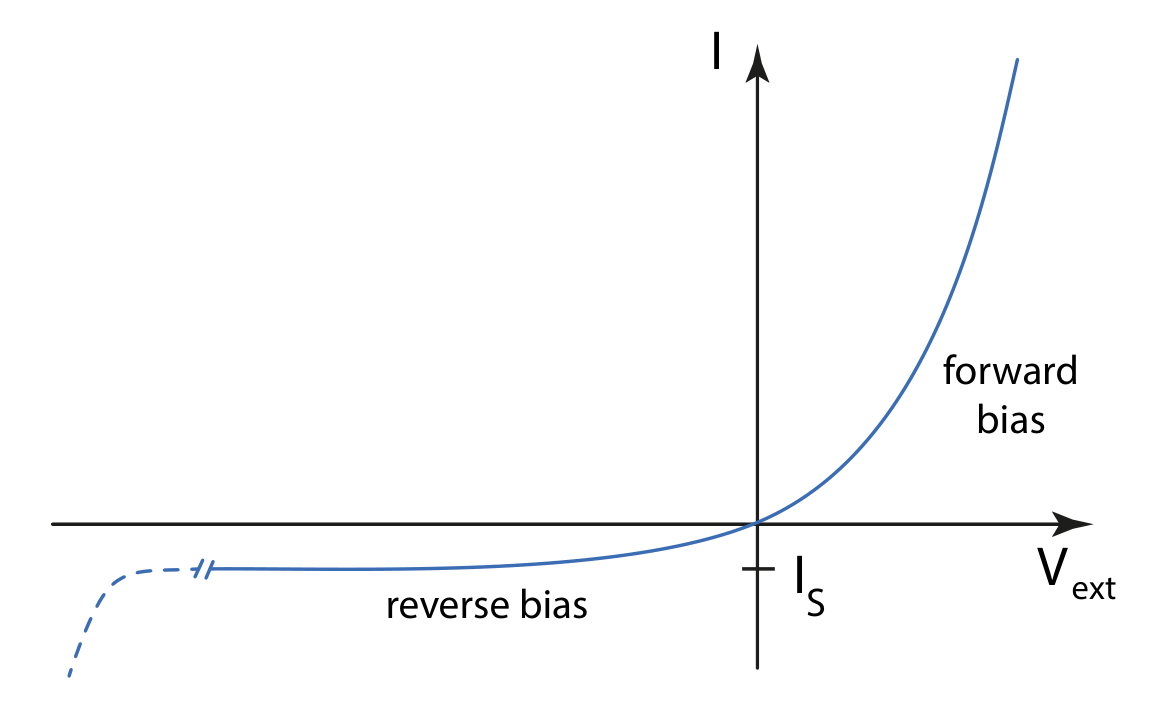
\includegraphics[width=0.5\textwidth]{figure/kennlinie}
	\caption[Schematic current--voltage characteristic of an ideal pn diode.]{Schematic current--voltage characteristic of an ideal pn diode under forward bias ($V_\text{ext} > 0$) and reverse bias ($V_\text{ext} < 0$).
		On the left-hand side of the reverse-bias curve, the characteristic I--V behavior of a pn diode is shown \cite{Moll}.}
	\label{fig:kennlinie}
\end{figure}

Conversely, when a reverse bias ($V_\text{ext} < 0$) is applied in the direction of the drift current,
the external electric field reinforces the existing space charge and increases the width of the depletion region.
For a fixed applied voltage, the width of the depletion region depends on the effective doping concentration \Cite{Moll}.

Electrons and holes
that diffuse into the depletion region under the influence of the electric field
usually recombine there.
Nevertheless, there is always a small number of charge carriers
that traverse the depletion region and induce a current.
This current is referred to as the \textit{leakage current}.
Assuming that no charge carriers are generated within the depletion region,
this current remains constant throughout the entire diode and is independent of the applied reverse bias.
Additional thermally generated electron--hole pairs can be created within the depletion region,
contributing to the leakage current.
An increase in the reverse bias also increases the leakage current,
since a wider depletion region allows more electron--hole pairs to be generated.
Once the applied reverse bias reaches a critical value, known as the \textit{breakdown voltage},
avalanche breakdown occurs,
causing the current to increase abruptly.
This is indicated by the dashed line in Figure~\ref{fig:kennlinie}.
At this point, the electric field within the depletion region is sufficiently strong
that electrons and holes acquire enough energy
to free additional charge carriers through impact ionization.
This process leads to a chain reaction,
resulting in an avalanche-like multiplication of charge carriers \cite{Bonn}.



\subsection{Silicon strip sensors}
Silicon strip sensors are semiconductor detectors that utilize the properties of silicon to detect ionizing radiation.
They consist of a thin layer of n-type silicon with embedded strips of p-type material.
An example of a silicon strip sensor is shown in \autoref{fig:strip_sensor}.
\begin{figure}[h]
	\centering
	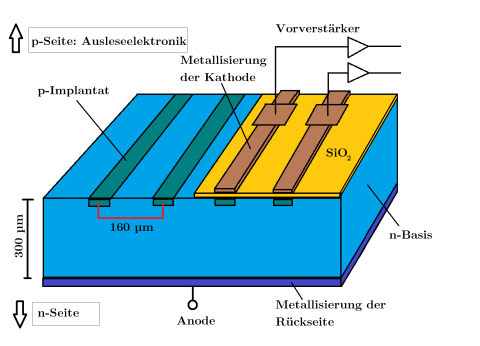
\includegraphics[width=0.5\textwidth]{figure/stripe.PNG}
	\caption[Schematic drawing of a silicon strip sensor.]{Schematic drawing of a silicon strip sensor \cite{Vorlage}.}
	\label{fig:strip_sensor}
\end{figure}
An external voltage is applied to the sensor, creating a depletion region between the n-type and p-type materials.
When ionizing radiation passes through the sensor, it generates electron-hole pairs in the depletion region.
The electric field within the depletion region seperates the electrons and holes, causing them to drift towards the respective electrodes.
The movement of the charge carriers induces a current in the electrodes, which can be measured and used to determine the energy of the incident radiation.

\subsection{Interaction with ionising radiation}
Ionising particles deposit their energy trough different processes in the material they traverse.
Therefor they are easily detectable.
The interactions that occur mainly are elastic collisions with the nucleus and collisions with the electrons of the atomic shell.
The energy loss on average per distance is described by the Bethe-Bloch formula \cite{Vorlage}:
\begin{equation}
	-\frac{dE}{dx} = K z^2 \frac{Z}{A} \frac{1}{\beta^2} \left[ \frac{1}{2} \ln{\frac{2 m_e c^2 \beta^2 \gamma^2 T_\text{max}}{I^2}} - \beta^2 - \frac{\delta(\beta\gamma)}{2} \right].
\end{equation} 
Here $\tau$ has the unit $m_ec^2$ and corresponds to the kinetic energy.
A overview of the parameters can be found in \cite{Vorlage}.

For thin silicon sensors, 
the deposited energy of traversing electrons cannot be described by a Gaussian distribution, 
since the sensor thickness is insufficient for the central limit theorem to apply. 
Additionally, 
some secondary electrons escape the sensor, 
resulting in an asymmetric energy distribution that resembles a Landau distribution. 
Since the electrons from the source are not monoenergetic,
the energy spectrum is best described by a convolution of a Gaussian and a Landau distribution. 
The most probable value of the energy loss is below the mean energy loss. 





